\documentclass{beamer}

\usepackage{beamer_tom}
\graphicspath{{/home/tom/Pictures/People/}{./images/}{./}}

\def\biblio{
    \nobibliography{../../library}
    \def\biblio{}
}

\institute{INRIA Saclay}
\author{Thomas Moreau}
\title{
    Flow-based Neural Posterior Estimation for Computational Imaging
}

\def\jointwork{Joint work with:
    P. Rodrigues, A. Gramfort, M. Jallais, D. Wassermann\\[1em]
    \includegraphics[height=5em]{prodriguez}
    \hskip5ex
    \includegraphics[height=5em]{agramfort}
    \hskip5ex
    \includegraphics[height=5em]{mjallais}
    \hskip5ex
    \includegraphics[height=5em]{dwassermann}
    \vskip-2.5em
   }

\setbeamertemplate{title page}[frame]
\def\extraLogo{}


\definecolor{palegreen}{RGB}{236,240,241}
\setbeamercolor{bgcolor}{fg=black!60,bg=palegreen}
\setbeamercolor{bordercolor}{fg=black!80,bg=darkblue}

\begin{document}

    \begin{frame}
        \titlepage
    %	\biblio{}
    \end{frame}

    \begin{frame}{Inverse problems}
        \begin{beamercolorbox}[wd=\textwidth, center, sep=.3ex]{separation line}
        \begin{beamercolorbox}[wd=.99\textwidth, center, sep=1ex]{headline}
            Inferring parameters of a model from observations is\\
            a fundamental scientific challenge.
        \end{beamercolorbox}
        \end{beamercolorbox}

        \begin{columns}[T]
            \column{.32\textwidth}
            Ion channel parameters\\
            \emph{e.g.} conductance.\\[.3em]
            \begin{beamercolorbox}[wd=\textwidth, center, sep=1ex]{bgcolor}
                Hodgkin-Huxley model\\
                (neuroscience)
            \end{beamercolorbox}
            Membrane potential

            \column{.32\textwidth}
            Epidemy parameters\\
            \emph{e.g.} $R_0$.\\[.3em]
            \begin{beamercolorbox}[wd=\textwidth, center, sep=1ex]{bgcolor}
                \vskip.5em
                SIR model\\
                (epidemiology)
                \vskip.5em
            \end{beamercolorbox}
            Number of infections

            \column{.32\textwidth}
            Physical quantities\\
            \emph{e.g.} particles energies.\\[.3em]
            \begin{beamercolorbox}[wd=\textwidth, center, sep=1ex]{bgcolor}
                \vskip.5em
                Standard model\\
                (particle physics)
                \vskip.5em
            \end{beamercolorbox}
            Measurements on colliders
        \end{columns}
        \vskip1em
        \begin{columns}[T]
            \column{.33\textwidth}
            \vskip2.2em
            \flushright%
            Parameters $\theta$%
            \column{.33\textwidth}
            \begin{beamercolorbox}[wd=\textwidth, center, sep=1ex]{bgcolor}
                Forward model $\mathcal M$\\
                $\rightarrow$
            \end{beamercolorbox}
            \begin{beamercolorbox}[wd=\textwidth, center, sep=1ex]{block title}
                Inverse model\\
                $\leftarrow$
            \end{beamercolorbox}
            \column{.33\textwidth}
            \vskip2.2em
            Observations $x$%
        \end{columns}
    \end{frame}

    \begin{frame}
        \frametitle{Likelihood-Free Inference (LFI)}

            \myitem We want to compute the posterior probability:
            \[
                p(\theta | x) = \frac{p(x | \theta) p(\theta)}{p(x)}
            \]
            where $p(x) = \int p(x | \theta) p(\theta)d\theta$\\[2em]

            \myitem Untrackable when the likelihood $p(x | \theta)$ is not analytic.\\[2em]

            \myitem In LFI, we trade analytic information for computational effort:

            \strongpoint{Approximate posterior with learning.}


    \end{frame}

    \begin{frame}
        \frametitle{Likelihood-Free Inference - Neural posterior Estimation}

        \begin{columns}
            \column{.6\textwidth}
                \myitem Sample parameters $\theta_i$ from prior $p(\theta)$,\\[1em]

                \myitem Simulate observation $x_i$ with forward model,\\[1em]

                \myitem Use $\{x_i, \theta_i\}$ to get an approximation of the posterior distribution.\\[1em]

                \hrule\vskip1em

                \myitem Posterior estimate is modeled using a normalizing flow $T$.
                \begin{align*}
                    u\sim \mathcal N(0, Id);&\quad x = T(u, \theta)\\
                        p(x | \theta) = p_{u, \theta}&\Big(T^{-1}(x)\Big) \Big| \det(J_{T^{-1}}(x))\Big|
                \end{align*}
                    \column{.4\textwidth}
            % \includegraphics[width=\textwidth,trim={15em 9em 7.3em 1em}, clip]{sbi_schematic}\\
            \includegraphics[width=\textwidth]{sbi_schematic2}\\

            {\centering [\emph{Lueckmann et al. 2021}]\\}

        \end{columns}


    \end{frame}

    \begin{frame}
        \frametitle{Application: diffusion MRI \rightcite{Jallais et al. 2021}}

        \begin{columns}
            \column{.25\textwidth}
            Infer Cytoarchitecture from diffusion MRI recordings.
            \column{.75\textwidth}
            \centering
            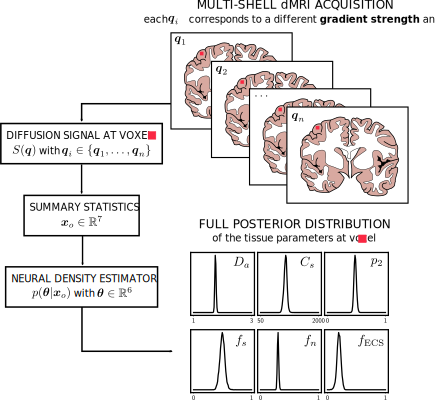
\includegraphics[height=.9\textheight]{sbi-dmri-pipeline}\\
        \end{columns}
    \end{frame}

    \begin{frame}
        \frametitle{Key challenge: Non-injective models}

        \begin{columns}
            \column{.25\textwidth}
            \centering
            \includegraphics[width=.5\textwidth]{mic}\\
            \column{.25\textwidth}
            \centering
            Distance
            \includegraphics[width=\textwidth]{arrow}
            \column{.25\textwidth}
            \centering
            Voice Amplitude
            \includegraphics[width=.5\textwidth]{speaker}
            \column{.25\textwidth}
            \visible<2>{
                \begin{beamercolorbox}[wd=\textwidth, center, sep=.3ex]{bordercolor}
                    \begin{beamercolorbox}[wd=.965\textwidth, center, sep=1ex]{darkbluebox}
                        Other speakers at same distance
                    \end{beamercolorbox}
                \end{beamercolorbox}
            }
        \end{columns}

        \begin{beamercolorbox}[wd=\textwidth, center, sep=.3ex]{separation line}
            \begin{beamercolorbox}[wd=.99\textwidth, center, sep=1ex]{headline}
                Close and quiet or far and loud?
            \end{beamercolorbox}
        \end{beamercolorbox}

        \begin{columns}
            \column{.25\textwidth}
            \centering
            \includegraphics[height=5em]{MEG_signals}
            \vskip-2em\hskip2ex
            \includegraphics[height=5em]{MEG_signals}
            \column{.25\textwidth}
            \centering
            Brain tissue\\
            \includegraphics[width=\textwidth]{arrow}\\
            propagation
            \column{.25\textwidth}
            \centering
            brain activity
            \includegraphics[width=.5\textwidth]{brain}\\
            \column{.25\textwidth}
            \visible<2>{

                \begin{beamercolorbox}[wd=\textwidth, center, sep=.3ex]{bordercolor}
                    \begin{beamercolorbox}[wd=.965\textwidth, center, sep=1ex]{darkbluebox}
                        Other recordings from the same subject
                    \end{beamercolorbox}
                \end{beamercolorbox}
            }
        \end{columns}
        \begin{beamercolorbox}[wd=\textwidth, center, sep=.3ex]{separation line}
            \begin{beamercolorbox}[wd=.99\textwidth, center, sep=1ex]{headline}
                Amplified weak or attenuated strong ?
            \end{beamercolorbox}
        \end{beamercolorbox}
        \visible<2>{
        \strongpoint{Global and local parameters: $\theta = (\alpha, \beta)$.}
        }
    \end{frame}

    \frame{
        \frametitle{Leveraging extra observations
                    \rightcite{Rodrigues et al. 2021}}


        Along with our observation $x_0$, we have $\mathcal X = \{x_1, \dots x_N\}$ extra observations that share a global parameter $\beta$.\\[1em]

        {\bf Factorized/Hierachical model:}
        \[
            p(\alpha, \beta | x_0, \mathcal X) = p(\alpha| \beta, x_0)p(\beta| x_0, \mathcal X)
        \]
        \vskip1em
        {\bf Key points}\\[.5em]
        \myitem Use factorized normalizing flow
        \[
            p(\alpha, \beta | x_0, \mathcal X) \approx
            q_{\phi_1}(\alpha|\beta, x_0) q_{\phi_2}(\beta|x_0, f_{\phi_3}(\mathcal X))
        \]
        \myitem Fit the flow using KL-divergence,\\[.5em]
        \myitem Use deep-set function for $f_{\phi_3}$ (permutation invariance).

    }

    \frame{
        \frametitle{Results: toy model $x = \alpha\beta$}

        \centering
        \includegraphics[height=.9\textheight]{ToyModel_nextra_100}\\
    }

    \frame{
        \frametitle{Results: Jansen \& Rit Neural Mass Model}

        {
            \centering
            \begin{columns}
                \column{.4\textwidth}
                \includegraphics[width=\textwidth]{JR_schematic}
                \column{.5\textwidth}
                \includegraphics[width=\textwidth]{JRNMM}\\
            \end{columns}
        }

        {\bf Parameters:}
        \begin{itemize}
            \item Mean $\mu$ and Variance $\sigma$ of spike train
            \item Internal connectivity $C$
            \item Gain factor $g$
        \end{itemize}
    }

    \frame{
        \frametitle{Results: Jansen \& Rit Neural Mass Model}

        \centering
        % \includegraphics[width=.5\textwidth]{indeterminacy}%
        \includegraphics[width=.7\textwidth]{determinacy}\\
    }

    \frame{
        \frametitle{Results: Jansen \& Rit Neural Mass Model}

        \centering
        \includegraphics[width=\textwidth]{alpha_rythm}\\
    }

    \frame{
        \frametitle{Results: Jansen \& Rit Neural Mass Model}

        \centering
        \includegraphics[height=.8\textheight]{alpha_rythm_params}\\
    }

    \frame{
        \frametitle{Conclusion}

        {\bf Take home messages}\\[1em]
        \begin{itemize}\itemsep1em
            \item LFI can be use to infer physical quantities from recordings.
            \item Normalizing flows are powerful tools to modelize posterior probabilities.
            \item Using mutliple recordings to solve indeterminacies can help obtain more statistical power.
        \end{itemize}
        \vskip2em
        {\bf References:}\\[.5em]
        Jallais, Rodrigues, Gramfort, Wassermann, \emph{Cytoarchitecture Measurements in Brain Gray Matter using Likelihood-Free Inference}, IPMI 2021\\[.5em]
        Rodrigues, {\bf M.}, Gramfort, \emph{Leveraging Global Parameters for Flow-based Neural Posterior Estimation}, preprint 2021.

    }

\end{document}